\section{一氧化碳}\label{sec:3-5}

碳的氧化物除二氧化碳外,还有一种叫做一氧化碳的氧化物。
在煤炉里(图 \ref{fig:3-10})煤层的上方常看到有蓝色火焰出现。这就是一氧化碳在燃烧。

一氧化碳(\ce{CO})分子虽然只比二氧化碳(\ce{CO2})分子少一个氧原子,
但是它们的性质却有很大的差别。

\begin{figure}[htbp]
    \centering
    \begin{minipage}[b]{7cm}
        \centering
        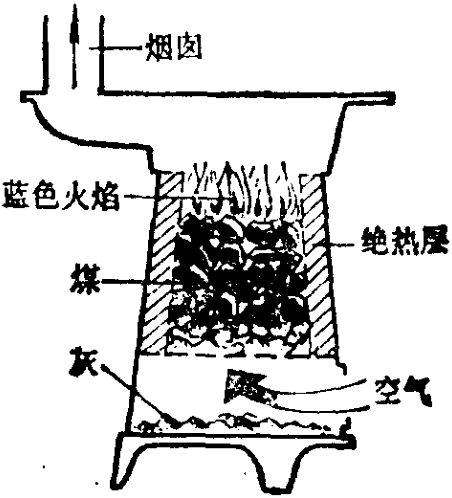
\includegraphics[width=4cm]{../pic/czhx1-ch3-10}
        \caption{煤炉简图}\label{fig:3-10}
    \end{minipage}
    \qquad
    \begin{minipage}[b]{7cm}
        \centering
        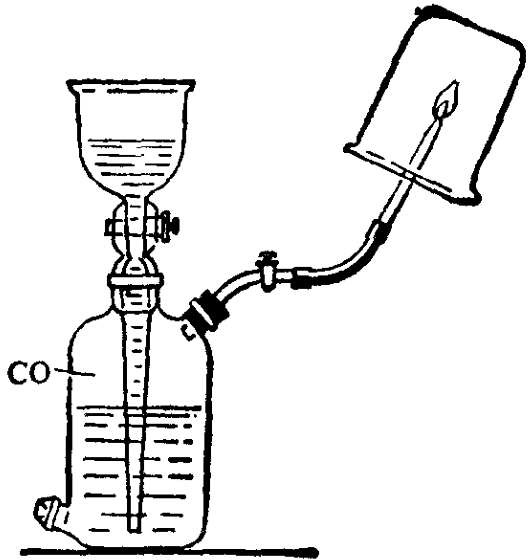
\includegraphics[width=4cm]{../pic/czhx1-ch3-11}
        \caption{一氧化碳的燃烧}\label{fig:3-11}
    \end{minipage}
\end{figure}

一氧化碳是一种没有颜色、没有气味的气体。在标准状况下,一氧化碳的密度是 $1.250 \; \kms$。
在通常状况下, 1 体积的水仅能溶解约 0.02 体积的一氧化碳。

一氧化碳有下列的主要化学性质:

\subsection{一氧化碳的可燃性}

\begin{shiyan}
    在盛有一氧化碳的贮气瓶的导管口点火,观察一氧化碳火焰的颜色。
    把杯璧附有澄清石灰水的烧杯罩在火焰上(图 \ref{fig:3-11}),观察石灰水有什么变化。
\end{shiyan}


一氧化碳在空气里能够燃烧,燃烧的时候发出蓝色的火焰,生成物是二氧化碳:
\begin{fangchengshi}
    \ce{ 2CO + O2 \xlongequal{\text{点燃}} 2CO2 }
\end{fangchengshi}

这个反应是放热反应。起反应的时候会放出大量的热。
因此,一氧化碳常常是许多气体燃料的主要成分。


\subsection{一氧化碳的还原性}

\begin{shiyan}
    按照图 \ref{fig:3-12} 的装置,往玻璃管里放入氧化铜粉末,加热, 然后通入一氧化碳。
    注意观察黑色氧化铜的变化和石灰水是不是变浑浊。
\end{shiyan}

\begin{figure}[htbp]
    \centering
    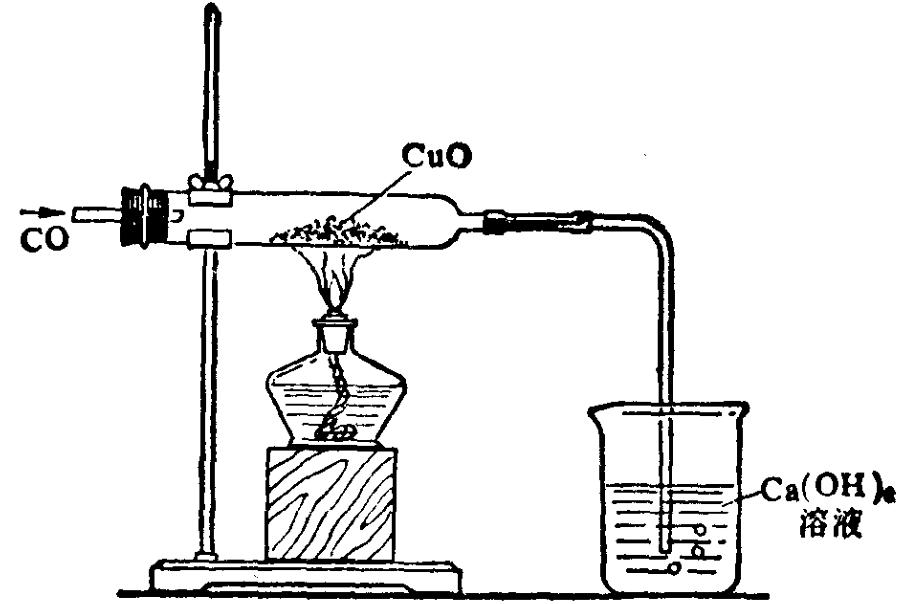
\includegraphics[width=8cm]{../pic/czhx1-ch3-12}
    \caption{一氧化碳使氧化铜还原成铜}\label{fig:3-12}
\end{figure}


黑色的氧化铜变成红色的铜,生成的气体是二氧化碳。

根据前面我们学过的关于氧化-还原反应的知识可知,
氧化铜里的氧被一氧化碳所夺取,氧化铜失去了氧,发生了还原反应;同时,
一氧化碳能够夺取氧化铜里的氧,一氧化碳得到了氧,发生了氧化反应。
所以在一氧化碳还原氧化铜的反应里,在发生还原反应的同时,也发生氧化反应。
人们通过大量的实验证明,氧化反应总是跟还原反应同时发生的。
下面我们分析在氧化铜跟一氧化碳的反应中有关元素化合价的变化。
这个反应可以用化学方程式表示如下(在各元素符号的上方注明了它们的化合价,并用线和箭头表示元素化合价的变化):

\begin{fangchengshi}
    \phantom{a} \\[0.5em]
    \ce{ CuO \; + \; CO \; = \; Cu \; + \; CO2 } % 按照原书的写法,使用 \; 加大间隔
    \tikz [overlay, >=Stealth] {
        \draw (-4.9, 0.45) node {\tiny $+2$};
        \draw (-4.4, 0.45) node {\tiny $-2$};
        \draw (-3.4, 0.45) node {\tiny $+2$};
        \draw (-3.0, 0.45) node {\tiny $-2$};
        \draw (-1.8, 0.45) node {\tiny $0$};
        \draw (-0.7, 0.45) node {\tiny $+4$};
        \draw (-0.3, 0.45) node {\tiny $-2$};
        \draw [->] (-3.3,  0.6) -- ++(0,  0.4) -- ++(2.7, 0) node [midway, above] {\small 化合价升高,被氧化} -- ++(0,  -0.4);
        \draw [->] (-4.8, -0.1) -- ++(0, -0.4) -- ++(3.0, 0) node [midway, below] {\small 化合价降低,被还原} -- ++(0, 0.4);
    }
    \\[1em]
\end{fangchengshi}

从上面的化学方程式里可以看出,氧化铜中铜的化合价由 $+2$ 价变成了铜单质中的 $0$ 价,
铜的化合价降低了,我们说氧化铜被还原了。
同时,一氧化碳中碳的化合价由 $+2$ 价变成了二氧化碳中的 $+4$ 价,
碳的化合价升高了,我们说一氧化碳被氧化了。

用化合价升降的观点来分析大量的氧化-还原反应可以得出以下的认识:

物质所含元素化合价升高的反应就是氧化反应,
物质所含元素化合价降低的反应就是还原反应。
凡有元素化合价升降的化学反应就是氧化-还原反应。
所含元素化合价升高的物质是还原剂,
所含元素化合价降低的物质是氧化剂。

用化合价升降的观点不仅能分析象氧化铜跟一氧化碳这类有失氧和得氧关系的反应,
还能分析一些没有失氧和得氧关系而发生元素化合价升降的反应。
让我们来分析钠跟氯气的反应。

\begin{fangchengshi}
    \phantom{a} \\[0.5em]
    \ce{ 2Na \; + \; Cl2 \; = \; 2NaCl }
    \tikz [overlay, >=Stealth] {
        \draw (-3.6, 0.45) node {\tiny $0$};
        \draw (-2.3, 0.45) node {\tiny $0$};
        \draw (-0.7, 0.45) node {\tiny $+1$};
        \draw (-0.3, 0.45) node {\tiny $-1$};
        \draw [->] (-3.6,  0.6) -- ++(0,  0.4) -- ++(2.9, 0) node [midway, above] {\small 化合价升高,被氧化} -- ++(0,  -0.4);
        \draw [->] (-2.3, -0.1) -- ++(0, -0.4) -- ++(2.1, 0) node [midway, below] {\small 化合价降低,被还原} -- ++(0, 0.4);
    }
    \\[1em]
\end{fangchengshi}


钠从 $0$ 价升高到 $+1$ 价,钠单质被氧化了;
氯从 $0$ 价降低到 $-1$ 价,氯气被还原了。
这个反应尽管没有失氧和得氧关系,但发生元素化合价的升降,因此也是氧化-还原反应。
在反应中钠是还原剂,而氯气是氧化剂。


\taolun 比较在钠跟氯气的反应前后,两种元素化合价发生的变化和两种原子核外电子的得失,
从这一事实当中可以得出这个氧化-还原反应里化合价的变化跟电子得失有什么关系。

氧化-还原反应常被用于工业生产上。由于一氧化碳具有还原性,在冶金工业里常用来作还原剂,
使金属氧化物发生还原以制取某些金属。例如,一氧化碳能在高温下还原铁矿石中的氧化铁,
同时生成二氧化碳。这个反应可以表示如下:
\begin{fangchengshi}
    \ce{ Fe2O3 + 3CO \xlongequal{\text{高温}} 2Fe + 3CO2 }
\end{fangchengshi}


\subsection{一氧化碳的毒性}

一氧化碳有剧毒。吸进肺里跟血液里的血红蛋白化合,使血红蛋白不能很好地跟氧气化合,人体就缺少氧气。
人吸入少量的一氧化碳就会感到头痛,吸入较多量的一氧化碳,就会因缺乏氧气而死亡。

由于一氧化碳没有颜色和气味,不容易被人察觉,所以对它要特别小心。
冬天用煤火取暖,如果不装烟囱或虽装烟囱而排气不良,常会发生煤气中毒事件,这就是中了一氧化碳的毒。

\begin{yuedu}
    空气里含少量的一氧化碳。在某些海洋面上,一氧化碳的含量只占百万分之 0.04 (常用 0.04 ppm 表示),
    而在一个拥挤的域市里,当无风的日子,地面上的一氧化碳含量可高达 360 ppm。
    含一氧化碳量在 50 ppm 以下的空气,被认为是安全的。
    如果一个人在空气中含一氧化碳量达 1000 ppm (即相当于每吸入 1000 体积空气中有 1 体积一氧化碳)的场合呆一会儿,
    就会感到头痛恶心,而当空气中一氧化碳含量达 10000 ppm 时,即使呆十分钟就会中毒死亡。

    居住拥挤的地区,空气里的一氧化碳主要是由于燃料没有充分燃烧和来自汽车排放出的废气。
    因此,我们应当重视一氧化碳对空气造成的污染问题。
\end{yuedu}


\begin{xiti}

\xiaoti{回答下列问题:}
\begin{xiaoxiaotis}

    \xxt{如果 \ce{CO} 中混有少量 \ce{CO2}, 怎样把 \ce{CO2} 除去?}

    \xxt{为什么 \ce{CO} 其有还原性,而 \ce{CO2} 没有还原性?}

\end{xiaoxiaotis}


\xiaoti{指出下列化合物里各元素的可变化合价。}
\begin{xiaoxiaotis}

    \begin{tblr}{columns={18em, colsep=0pt}}
        \xxt{\ce{SO2}、\ce{SO3};} & \xxt{\ce{FeO}、\ce{Fe2O3};} \\
        \xxt{\ce{Cu2O}、\ce{CuO};} & \xxt{\ce{NO}、\ce{NO2}。}
    \end{tblr}
\end{xiaoxiaotis}


\xiaoti{写出下列反应的化学方程式。根据反应前后元素化合价的升降来判断哪一种物质被氧化了,
    哪一种物质被还原了,哪一种物质是氧化剂,哪一种物质是还原剂。
}
\begin{xiaoxiaotis}

    \xxt{一氧化碳在空气中燃烧,}

    \xxt{氧化铅(\ce{PbO}) 跟氢气反应,}

    \xxt{氧化铅跟一氧化碳反应,}

    \xxt{氧化银(\ce{Ag2O}) 跟一氧化碳反应。}

\end{xiaoxiaotis}

\end{xiti}


